\section{Computational Fluid Dynamics for Aerodynamic Force Modeling}
\label{methods}
The objective of this section is to build models for the aerodynamic force $\boldsymbol{F_a}$ to be then considered in \eqref{eq:centroidal_momentum_dynamics} and \eqref{eq_motion}. In general, the aerodynamic force is hard to predict. It depends on the robot relative velocity, joint angles, and robot base orientation, thus rendering the overall task hard to solve. For this reason, this section performs \emph{Computational Fluid Dynamics} (CFD) simulations considering the robot as a \emph{single rigid body}, namely, the robot is kept with a specific joint configuration $\bar{s}$, and the following assumption is made.

\textbf{Assumption 1}: Assume a constant robot base and wind velocity. Given a robot joint configuration $\bar{s}$,
 the aerodynamic force is constant 
%\st{aerodynamic characteristics are consistent} 
when $s$ belongs to the neighborhood of $\bar{s}$.

The assumption above will be enforced by the design of flight controllers that keep the robot joints close to a specific configuration during flight.   
  
  
\subsection{CFD simplified robot model}
\label{sec:cfdModel}
 Considering \textbf{Assumption 1}, CFD simulations are all performed with fixed robot initial joint positions, which is supposed to been optimized given a flight metric (e.g. minimisation of thrust forces).
 Furthermore, a complex-shaped geometry as the iRonCub one can cause difficulties in the meshing phase of CFD simulations, because of errors caused by interference among complex parts. Therefore, 
 %\st{without losing the main geometrical characteristics of the robot}
 %\antonellosays{Probably we could change this sentence because we are changing a lot the geometry but we could state that this has not to affect the entire framework since the aerodynamic model can simply scale when substituted after performing simulations with a more accurate model in a future phase}, 
 we approximate the geometry of iRonCub representing the major robot links as simple cylinders (see Fig.~\ref{fig:notation}). The model allows to obtain high-quality meshes with a relatively low number of elements, which in turn translates in a reduction of the simulation time.
 
\subsection{Aerodynamic components for CFD analysis}
\label{sec:cfd} 
For the sole purpose of CFD analysis, let us introduce the frame $\mathcal{A}=\{{}^{\mathcal{I}}o_{\mathcal{G}};\boldsymbol{i}_a,\boldsymbol{j}_a,\boldsymbol{k}_a\}$ as the \emph{relative velocity} frame. It is defined for CFD simulations only, where the relative velocity is always different from zero, namely $|\boldsymbol{v}_a|\neq 0$. 
The $\boldsymbol{j}_a$ axis therefore aligns to the opposite direction of $\boldsymbol{v}_a$ (see also Fig. \ref{figureRelativeVelocityFrameCFD}).

\begin{figure}[t]
      \centering
      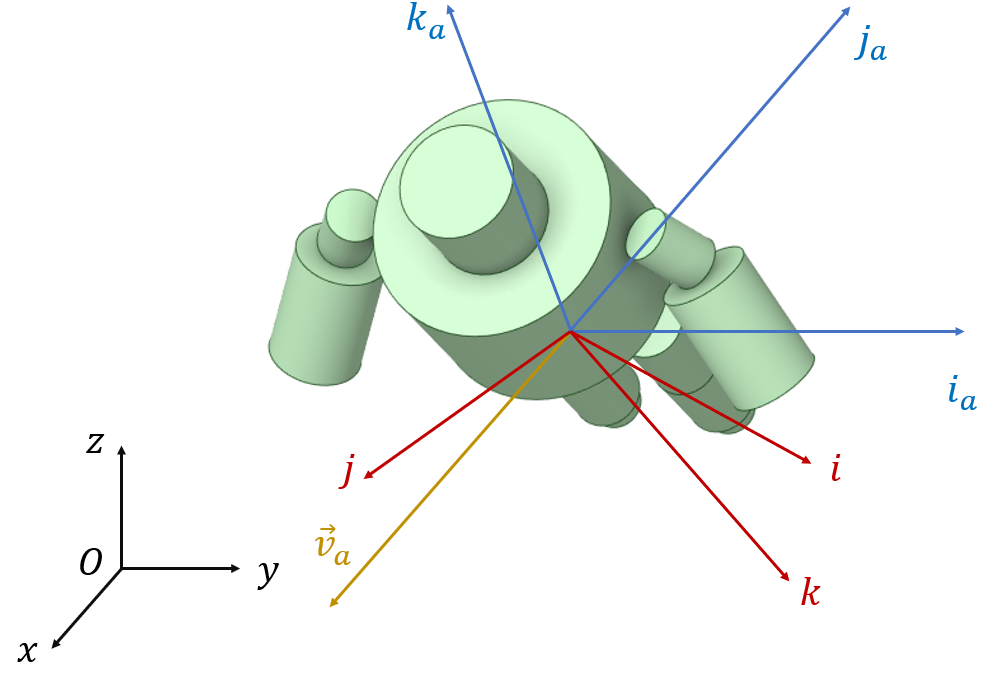
\includegraphics[width=60mm]{./imagines/CFD_Reference_System_3.png}
      \caption{CFD Model with the relative velocity frame.}
      \label{figureRelativeVelocityFrameCFD}
   \end{figure}

Then, we decompose the aerodynamic force w.r.t. the relative velocity frame $\mathcal{A}$ as:
\begin{equation}
\label{eq:af_total_control}
\boldsymbol{{F}_a}=\boldsymbol{{F}_D}+\boldsymbol{{F}_S}+\boldsymbol{{F}_N} ,
\end{equation}
where:
\begin{itemize}
    \item $\boldsymbol{{F}_D}$, the drag force, aligns to $\boldsymbol{j}_a$ axis;
    \item $\boldsymbol{{F}_S}$, the defined sideforce, aligns to $\boldsymbol{i}_a$ axis;
    \item $\boldsymbol{{F}_N}$, the defined normal force, aligns to $\boldsymbol{k}_a$ axis.
\end{itemize}
The intensity of the steady aerodynamic force varies approximately with $|\boldsymbol{v}_a|^2$, hence there exist three dimensionless functions $C_D$, $C_S$, $C_N$ depending on the Reynolds number $Re$, the Mach number $\mathcal{M}$ and $(\alpha, \beta)$, such that \cite{c3}\cite{c5}:
\begin{subequations}
\begin{align}
    \boldsymbol{{F}_D} & :=\mathcal{K}_a|\boldsymbol{v}_a|^2C_D(Re, \mathcal{M}, \alpha, \beta)\boldsymbol{j}_a,\\
    \boldsymbol{{F}_S} & :=\mathcal{K}_a|\boldsymbol{v}_a|^2C_S(Re, \mathcal{M}, \alpha, \beta)\boldsymbol{i}_a,\\
    \boldsymbol{{F}_N} & :=\mathcal{K}_a|\boldsymbol{v}_a|^2C_N(Re, \mathcal{M}, \alpha, \beta)\boldsymbol{k}_a,
\end{align}
\label{eq:af_coe}
\end{subequations}
\noindent with the angles $(\alpha, \beta)$ characterizing the relative orientation of $\boldsymbol{v}_a$ w.r.t. the body frame $\mathcal{D}$, chosen as in  Fig.~\ref{fig:notation}. So, $\alpha \in [0,\pi]$ is defined as the angle between $\boldsymbol{v}_a$ and the negative $\boldsymbol{k}$ axis of the body frame $\mathcal{D}$, while $\beta \in [0,2\pi]$ is defined as the angle between the projection of $\boldsymbol{v}_a$ on plane $(\boldsymbol{i},\boldsymbol{j})$ and the positive $\boldsymbol{i}$ axis of frame $\mathcal{D}$ (see also \cite{c3}). The constant $\mathcal{K}_a:=\frac{A_{ref}\rho}{2}$ with $\rho$ the air density and $A_{ref}$ the reference frontal area, moreover, $A_{ref}$ has been defined to obtain $\mathcal{K}_a = 1$ to simplify the calculation. Furthermore, we hereafter assume that the dependency upon the Mach and Reynolds numbers is negligible, and thus omitting these dependencies in the arguments of the aerodynamic coefficients.

\subsection{CFD results and simplified aerodynamic model}\label{sec:aeroModel}

Significant robot flight configurations, corresponding to precise values of $\alpha$ and $\beta$, were simulated using CFD tools. In total 45 simulations were run, with $ \alpha \in (\ang{15},\ \ang{30},\ \ang{45},\ \ang{60},\ \ang{90},\ \ang{120},\ \ang{150},\ \ang{160},\ \ang{180})$ and $ \beta \in (\ang{90},\ \ang{135},\ \ang{180},\ \ang{225},\ \ang{270})$ which supplied the necessary data for proceeding with the modeling of aerodynamic characteristics on iRonCub. Settings of CFD simulations are schematically reported in Table \ref{table:cfd}.

\begin{table}[t]
\caption{CFD simulation settings}
\label{table:cfd}
	\centering
	\begin{tabular}{c|l}
	    \toprule
	    \multirow{6}{*}{\textit{Solver Settings}} & Pressure--Velocity Coupling for \emph{RANS} \\ & (Reynolds Averaged Navier-Stokes) \\ & Steady-State Simulation\\ & SST $k - \omega$ for Turbulence modelling \\ & No Compressibility Effects \\ & (i.e. $M\ll1$, $\rho = \text{const}$)\\
		\midrule
		\multirow{2}{*}{\textit{Constant Values}} & Air density: $\rho = \SI{1.225}{kg/m^3}$ \\ & Reference pressure: $p_{ref} = \SI{1}{atm}$\\
        \midrule
        \multirow{3}{*}{\textit{Boundary Conditions}} & Inlet velocity: $v = \SI{7.5}{m/s}$ \\ & Outlet pressure: $p_{rel} = \SI{0}{Pa}$\\ & Walls: \textbf{No Slip} Condition\\
		\bottomrule
	\end{tabular}
\end{table}
\looseness=-1

As introduced in Sec. \ref{sec:cfd}, the three dimensionless functions $C_D$, $C_S$, $C_N$ are the aerodynamic characteristics of the body, i.e. the defined aerodynamic coefficients (AC): drag coefficient, sideforce coefficient and normal force coefficient. In this section, the analytical model of AC is identified based on the CFD results from Sec. \ref{sec:cfd}. To proceed with identification, the following assumptions are made:

\begin{enumerate}
\item the aerodynamic forces act at the robot's CoM (coincides with CoP) and therefore the aerodynamic moments ${M}_a$ are equal to zero;
\item from CFD results, the sideforce effect is neglected due to its small magnitude compared with the other two aerodynamic force components, and with other forces acting on the robot;
\item the AC dependence from Mach number $\mathcal{M}$ is considered negligible since the relative velocity intensity of the robot is much smaller than the sound speed (i.e. the density can be assumed as constant);
\item the AC dependence from Reynolds number $Re$ is not considered since the AC evaluated from CFD for different values of relative velocity doesn't show a significant dependence from it;
\item the effects of rotational and unsteady motions of the vehicle on its surrounding airflow are negligible~\cite{c5}.
\end{enumerate}

As a consequence, the AC depend only on the flight configuration $(\alpha,\beta)$ and can be written as~\cite{c3}:
\begin{equation*}
    C_D(\cdot) =C_D(\alpha, \beta), \quad  C_N(\cdot) =C_N(\alpha, \beta) .
\end{equation*}

Considering that the aerodynamic coefficients are naturally $2\pi$-periodic \cite{c12}, $\sin{(\cdot)}$ functions are used to design the mathematical models of AC: %, which are hereafter displayed:
\begin{equation}
    \resizebox{.88 \columnwidth}{!}{$ 
        C_D(\alpha,\beta)= c_0 + c_1 \sin{^2 \alpha} \sin{^2\beta} + c_2 \sin{^2\alpha}  + c_3 \sin{^2\beta}
    $},\label{eq:drag}
 \end{equation}
 \begin{equation}
    C_N(\alpha,\beta)= d_0 + d_1 \sin{^2\alpha} \sin{(2\alpha)} \sin{^2\beta} .
    \label{eq:normal}
 \end{equation}

The coefficients characterizing the expressions of $C_D(\cdot)$ and $C_N(\cdot)$:
\begin{itemize}
    \item $c_0=0.1274$, $c_1=0.0903$, $c_2=0.0141$, $c_3=0.0147$;
    \item $d_0=0.0007$, $d_1=0.0938$,
\end{itemize}
\noindent
are obtained using linear regression. \\
In fluid dynamics, drag force is a type of friction that acts in the opposite direction of the relative motion of any object moving in a fluid. Therefore the estimated drag coefficient $C_D$ should remain positive in the whole range of $\alpha$ and $\beta$. This property is verified by the identified model in Eq.~\eqref{eq:drag}, as Fig.~\ref{fig:drag model} shows.

As previously mentioned, the zero sideforce assumption allows the identification of the lift force with the normal force, as demonstrated in~\cite{c3} for axisymmetric bodies, since the normal component of the aerodynamic force lies on the $\boldsymbol{v}_a-\boldsymbol{k}_a$ plane. The aerodynamic forces acting on the robot CoM rewrite as:

\begin{equation}
\label{eq:aerodyModelSymmetricBodies}
\begin{array}{lcl}
	\boldsymbol{F_L} & = & k_a|\boldsymbol{v}_a|C_L(\alpha,\beta)\boldsymbol{r}(\beta) \times \boldsymbol{v}_a, \\
	\boldsymbol{F_D} & = & -k_a |\boldsymbol{v}_a|C_D(\alpha,\beta)\boldsymbol{v}_a, \\
\end{array}
\end{equation}
where  $\label{eq:aerodynamicsAuxiliaryVector}
\boldsymbol{r}(\beta)  =  -\sin(\beta) \boldsymbol{i}+\cos(\beta) \boldsymbol{j}.$

 \begin{figure}[t]
\centering
\subfigure[\label{fig:drag model}]{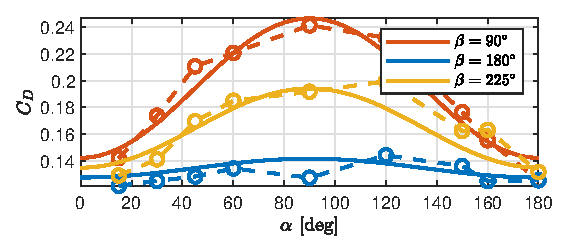
\includegraphics[width=0.97\columnwidth]{imagines/Cd_alpha.eps}}\\
\subfigure[\label{fig:normal model}]{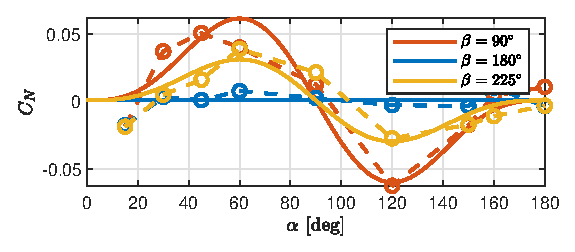
\includegraphics[width=0.97\columnwidth]{imagines/Cn_alpha.eps}} \\
\caption{AC models identified from CFD simulations data. Dashed lines represent the collected CFD data, solid lines represent the identified models.}
\label{fig:subfig}
\end{figure}

\section{Control Design}
\label{sec:control}

\subsection{Flight Control Without Aerodynamics Awareness}
\label{subsec:Flight-Control-no-aerodyn-forces}
The iRonCub flight controller~\cite{c1, c2} is a \emph{task-based} control strategy, composed of several control objectives (tasks), with different priorities. The so-called \emph{primary task}, i.e. the task with the higher priority, is the stabilization of the robot's \emph{centroidal momentum}\footnote{The centroidal momentum is the robot total momentum expressed w.r.t. the frame $\mathcal{G}[\mathcal{I}]$  defined in Sec. \ref{background}.} dynamics, which equals the summation of all external forces acting on the robot:
%
\begin{equation}
\label{eq:hdot}
   {}^{\mathcal{G}[\mathcal{I}]}\dot{\boldsymbol{h}}=\boldsymbol{A}(q)T+m\bar{\boldsymbol{g}}=f_h(q,T),
\end{equation}

%change f(q,T) to f_h(q,T), because f has been used as trust function, $g$ is the norm of gravitational acceleration and 
where $m$ is the robot's total mass, $\boldsymbol{A}(q) \in \mathbb{R}^{6 \times m}$ is a proper matrix mapping the thrust vector $T$ in the momentum equation. For the momentum control design, we assume that the robot joints velocities $\dot{s}$ and the thrust rate of change $\dot{T}$ can be chosen at will, and then can be considered as our control inputs. Therefore, we define $u := (\dot{T}, \dot{s})$. To make the control input $u$ appear in the momentum equation \eqref{eq:hdot}, we increase the relative degree of the output and write the momentum acceleration:
%
\begin{equation}
\label{eq:hddot}
   {}^{\mathcal{G}[\mathcal{I}]}\ddot{\boldsymbol{h}}=\dot{\boldsymbol{A}}(q)T+\boldsymbol{A}(q)\dot{T} = f_h(q, T, v, \dot{T}).
\end{equation}
%
As demonstrated in our previous works \cite{c1,c2}, it is possible to find a smooth control input $u^*$ that renders the closed-loop equilibrium point $(\dot{\tilde{\boldsymbol{h}}}, \tilde{\boldsymbol{h}}, \boldsymbol{I}) = (\boldsymbol{0},\boldsymbol{0},\boldsymbol{0})$ globally asymptotically stable, where $\tilde{\boldsymbol{h}} = \boldsymbol{h}-\boldsymbol{h}^d$, $\boldsymbol{h}^d$ is the reference momentum trajectory and $\boldsymbol{I} := \int_0^t \tilde{\boldsymbol{h}}$. 

We also define a \emph{postural task} to resolve the redundancy in the control input $u$ and maintain the robot configuration close to a desired shape:
%
\begin{equation}
\label{eq:postural}
   \dot{s}^* = -K_P^s (s-s^d),
\end{equation}
%
with $s^d$ the desired robot posture and $K_P^s \in \mathbb{R}^{n \times n}$ a positive gains matrix. The two tasks are then achieved by means of Quadratic Programming (QP) optimization framework:
\begin{IEEEeqnarray}{LLL}
\IEEEyesnumber
\label{eq:optimization_QP}
   u^{**} &=& \text{argmin}_{u} (w_1|u-u^*|^2 + w_2|\dot{s}-\dot{s}^*|^2) \\
     & s.t. & \qquad u_{min} \leq u \leq u_{max}, \nonumber
\end{IEEEeqnarray}
where \emph{soft} task priorities are assigned to the two tasks via proper weights $w_1, w_2 >0$. Framing the problem as an optimization procedure allows to include input boundaries $u_{min}, u_{max}$ in the control design. It is also possible to include the integral of input boundaries (namely, the joint position and thrust limits) in the QP design. For more details on these aspects of the flight control design, which are not relevant for this paper, we refer to previous works \cite{c1,c2}.

\subsection{Flight Control with Aerodynamics Awareness}

The flight controller discussed in \ref{subsec:Flight-Control-no-aerodyn-forces} does not consider the effect of aerodynamic forces. This missing information may impair the performances of the control algorithm when aerodynamic forces are not negligible. To overcome this limitation, we implemented two modifications of the iRonCub flight controller: \emph{feedback linearization} and \emph{gain scheduling}.
To implement our control strategy, we considered the following \textbf{Assumption 2}: we assume that $\dot{\boldsymbol{F}}_a = 0$ in the calculation of the momentum acceleration.

\subsubsection*{Addition of Aerodynamics Forces}
First, we include the estimated aerodynamic forces, obtained by writing Eq. \eqref{eq:af_total_control} with the aerodynamic coefficients estimated in Sec. \ref{sec:aeroModel}, in the robot equations of motion Eq. \eqref{eq_motion} and momentum dynamics Eq. \eqref{eq:hdot}, which renders:
\begin{equation}
\label{eq_motion_af}
  M(q)\dot{v}+C(q,v)v+G(q)=
  \begin{bmatrix}
    0_6\\
    \tau
  \end{bmatrix}
  +f(q,T)+J_{CoM}^{\top}F_a,
\end{equation}
where $J_{CoM} \in \mathbb{R}^{3 \times n+6}$ is the CoM Jacobian, while the momentum rate of change is now given by:
\begin{equation}
\label{eq:hdot_af}
   {}^{\mathcal{G}[\mathcal{I}]}\dot{\boldsymbol{h}}=\boldsymbol{A}(q)T+m\bar{\boldsymbol{g}}+
   \begin{bmatrix}
   \boldsymbol{F_a}\\
   0_3
   \end{bmatrix}.
\end{equation}

\subsubsection*{Feedback Linearization Control}

We assume that the relative velocity ${}^{\mathcal{I}}\boldsymbol{v}_a$ can be measured, for example by employing dedicated sensors such as Pitot tubes applied on the robot, allowing the computation of the aerodynamic force $F_a$. A feedback linearization controller then substitutes Eq.~\eqref{eq:hdot} with Eq.~\eqref{eq:hdot_af} in the calculation of the baseline control input $u^*$, which depends on the momentum rate of change $\dot{h}$. In this way we can cancel out the effects of the aerodynamic forces on the desired closed-loop momentum acceleration.

\subsubsection*{Implementation of Gain Scheduling}

if it is not possible to compute the aerodynamic forces with enough accuracy, gain scheduling is employed as a strategy to react to wind gusts. In particular, we assume that a wind gust is detected when the measured center of mass position error overcomes a certain threshold.

The desired closed-loop momentum acceleration has the following shape, which is obtained by applying the baseline controller $u^*$ Eq. \eqref{eq:optimization_QP}:
\begin{equation}
\label{eq:hddot_des}
   \ddot{\boldsymbol{h}} = \ddot{\boldsymbol{h}}^d -K_D\dot{\tilde{\boldsymbol{h}}} -K_P\tilde{{\boldsymbol{h}}} -K_I \boldsymbol{I}.
\end{equation}
When a wind gust is detected, gain scheduling smoothly increases the value of the gain $K_I$ and $K_P$, to guarantee a stronger response of the controller to the associated errors.